\documentclass{beamer}
\usepackage{config}

%Information to be included in the title page:
\title[Git seul en local mono-branche (Bonus)]{Git : mode d'emploi pour un usage seul, sans dépôt distant, sur une seule branche\\ (Bonus)}
\author{Florian Legendre}
\institute{Université de Poitiers}
\date{Année 2020 - 2021}
\logo{
\includegraphics[scale=0.1]{UP.png}}


%%% ============================================================= %%%
%%% ====================== Début des diapos ===================== %%%
%%% ============================================================= %%%

\begin{document}

\frame{\titlepage}

\begin{frame}
\frametitle{Table of Contents}
\tableofcontents[hideallsubsections]
\end{frame}


%% --------------------- %%
%%        SECTION        %%
%% --------------------- %%
\section{Commande: git revert <id>}

%% --------------------- %%
%%         BONUS         %%
%% --------------------- %%

\begin{frame}
\huge
\begin{center}
\hrule
\bigskip
Bonus\footnote[frame]{Partie optionnelle: revenez-y après avoir utilisé Git quelques-temps et avoir géré des conflits en travaillant à plusieurs} sur la commande\\ \textit{git revert <id>}
\bigskip
\hrule
\end{center}
\normalsize
\end{frame}

\begin{frame}{Commande: git revert <id>}
Si vous voulez annuler les changements apportés par une seule version en particulier vous pouvez le faire avec la commande \textit{git revert <id>}. Cependant, il est possible que vous ayiez à résoudre des conflits!\\
\medskip

En effet, \textit{git revert} annule un changement donné d'une version donnée en faisant l'inverse de ces-derniers dans votre dossier de travail. Or si Git trouve dans votre dossier de travail une valeur autre que celle présente dans la version choisie, Git ne saura pas s'il doit annuler cette modification aussi ou s'il doit conserver votre modification.
\end{frame}

\begin{frame}{Commande: git revert <id>}
On pose le fichier suivant (ce fichier fait l'objet d'un commit):
\begin{center}
	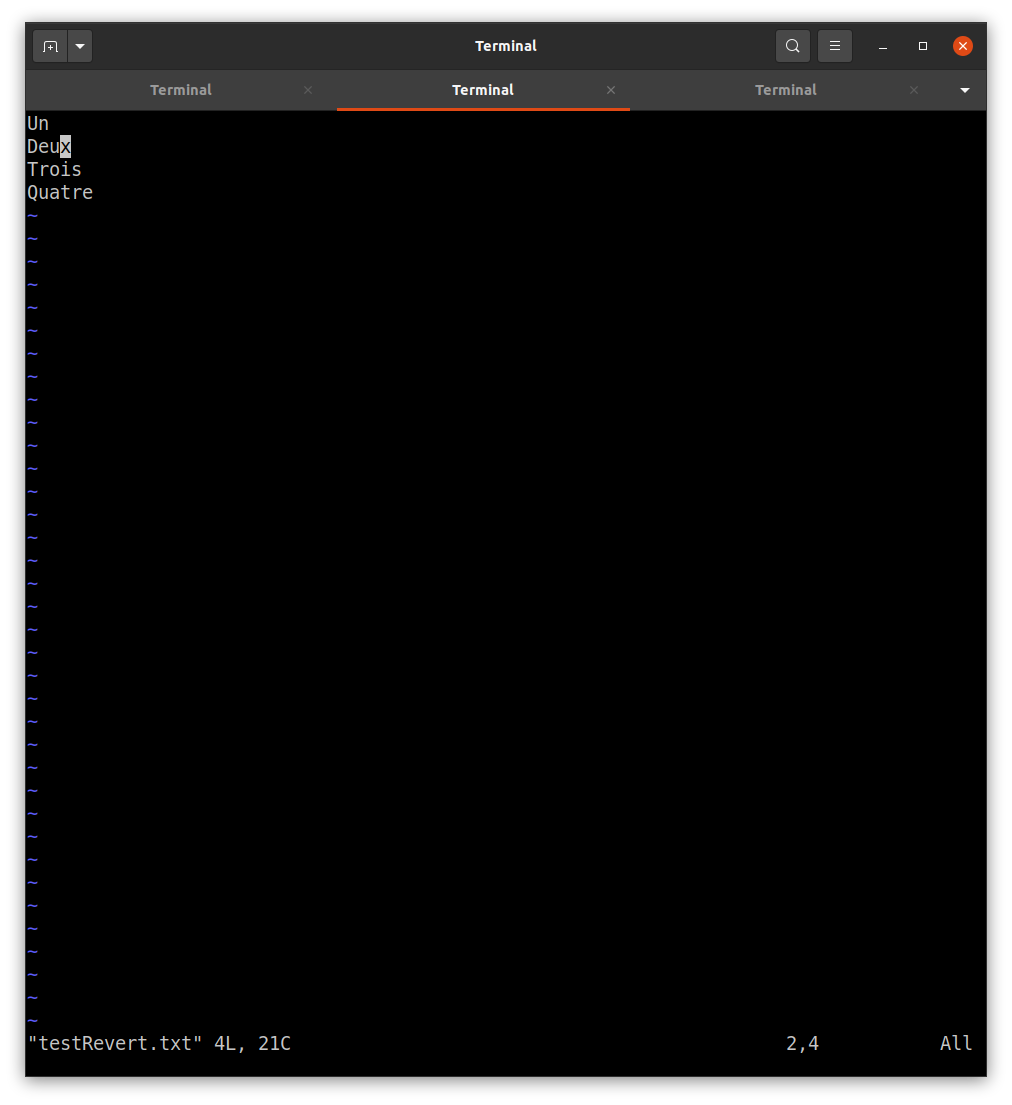
\includegraphics[scale=0.15]{gitRevert/gitRevert1.png}
\end{center}
\end{frame}

\begin{frame}{Commande: git revert <id>}
On remplace 'Deux' par le chiffre '2' et on commit:
\begin{center}
	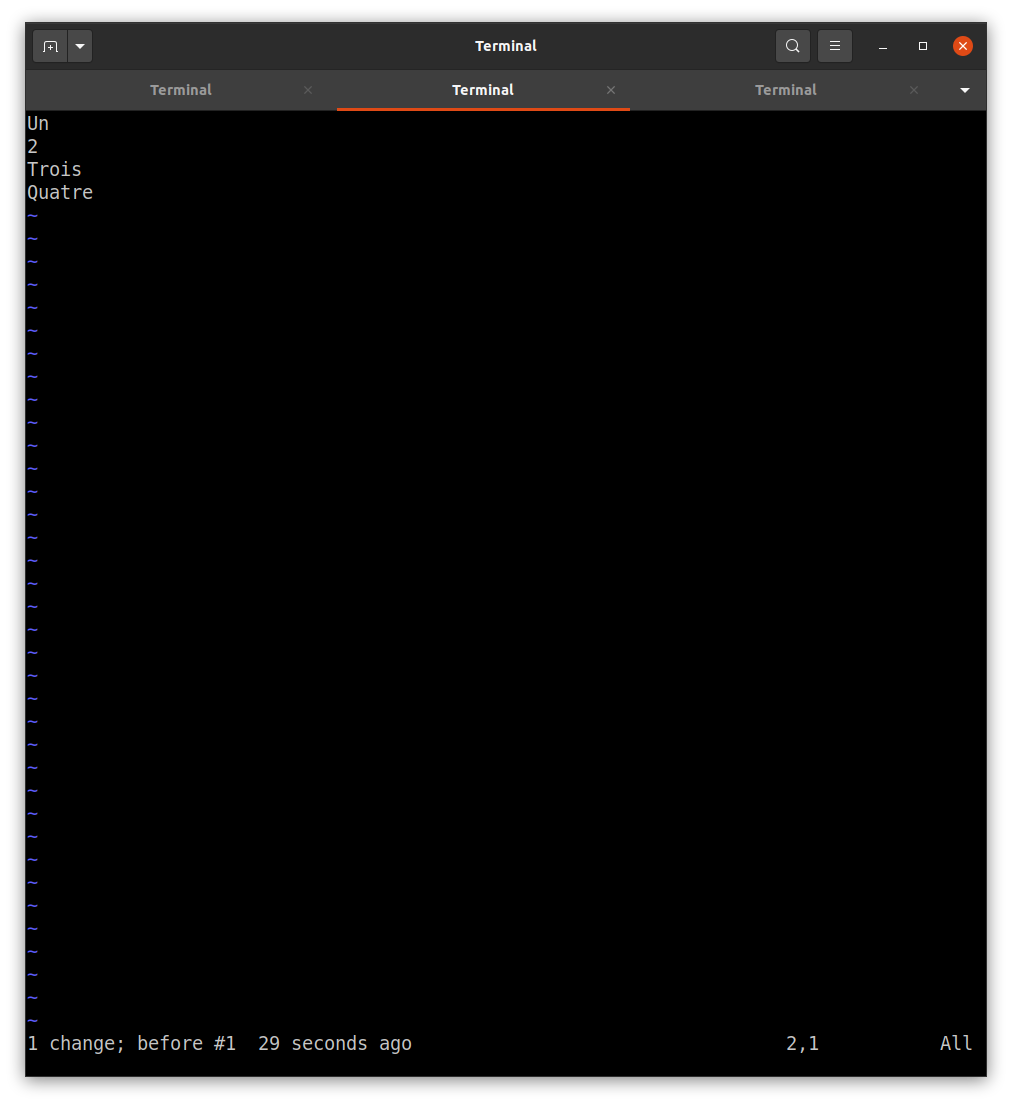
\includegraphics[scale=0.15]{gitRevert/gitRevert2.png}
\end{center}
\end{frame}

\begin{frame}{Commande: git revert <id>}
On obtient donc les deux versions suivantes:
\begin{center}
	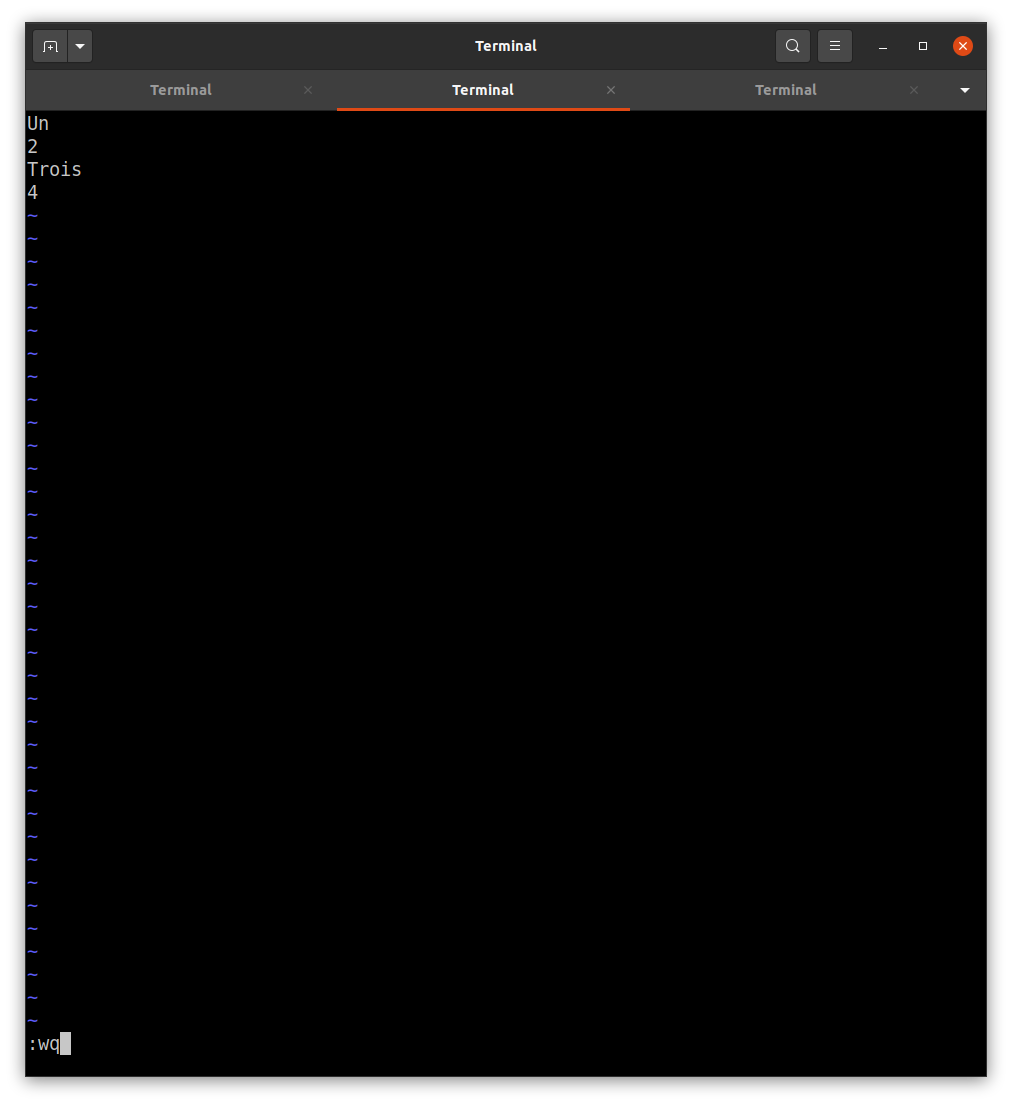
\includegraphics[scale=0.15]{gitRevert/gitRevert3.png}
\end{center}
\end{frame}

\begin{frame}{Commande: git revert <id>}
On essaye de "revert" le tout dernier commit, ie. là où se trouve notre tête "HEAD". Ce "revert" se déroule sans problème:
\begin{center}
	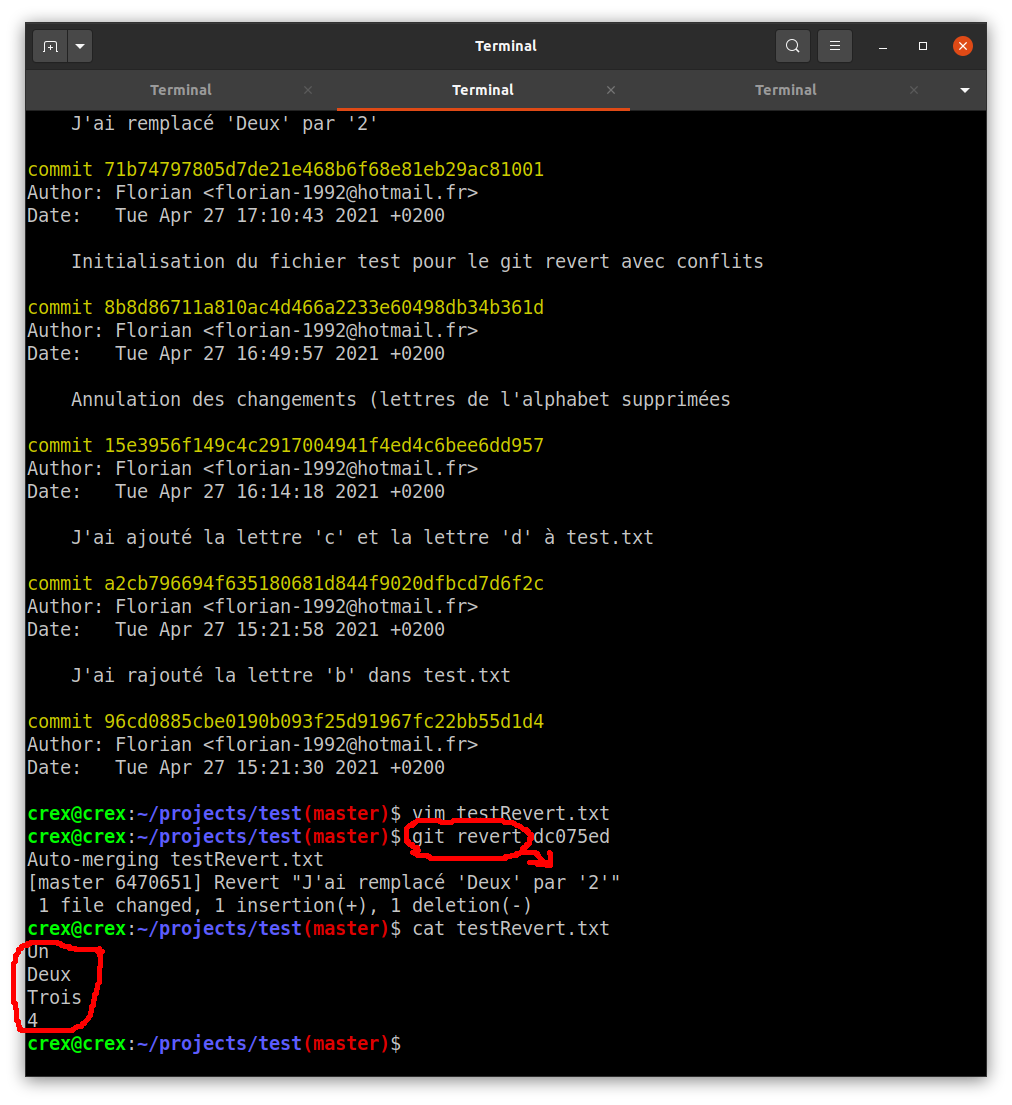
\includegraphics[scale=0.15]{gitRevert/gitRevert4.png}
\end{center}
\end{frame}

\begin{frame}{Commande: git revert <id>}
Le résultat est un fichier où '2' a été remplacé par 'Deux'. Git a fait l'inverse du changement indiqué par la version passée en paramètre:
\begin{center}
	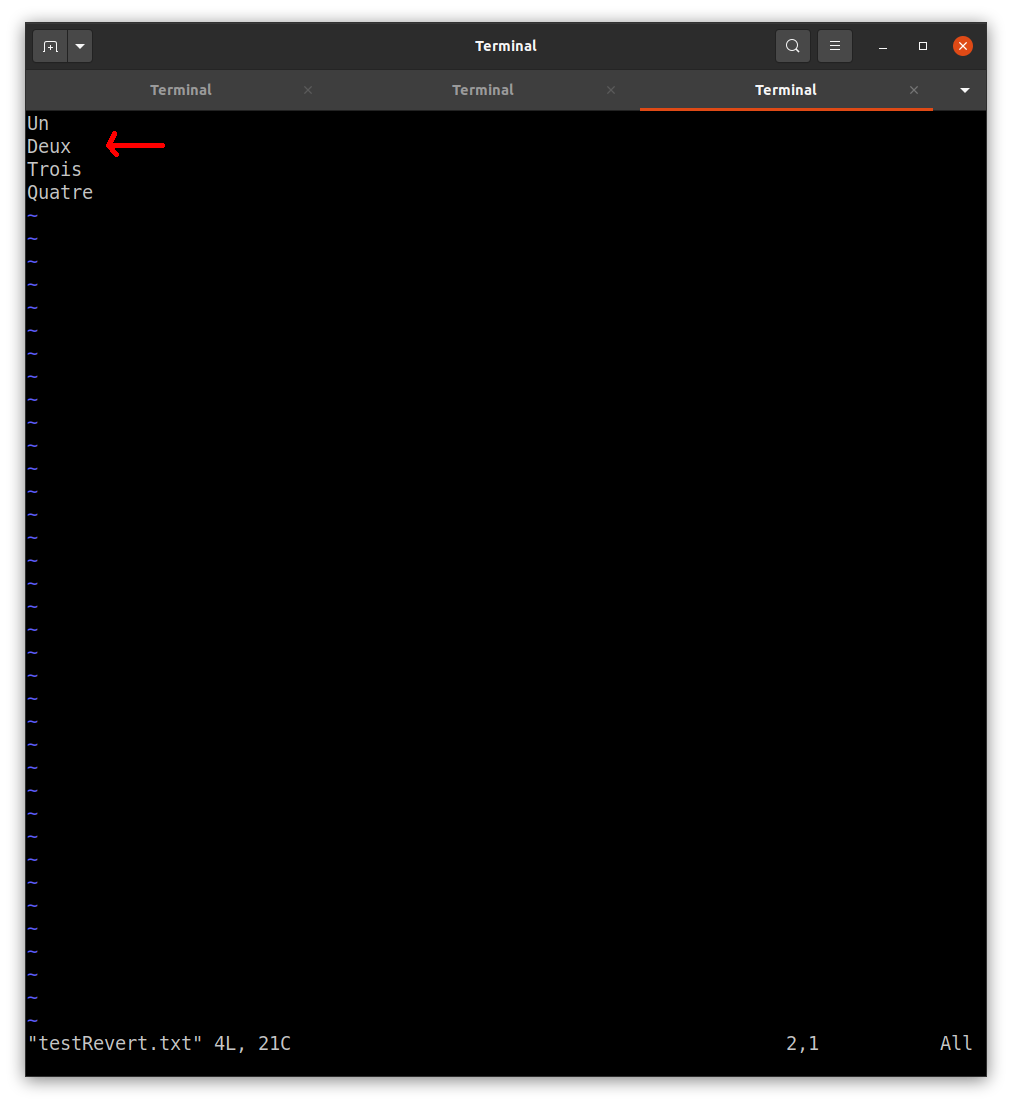
\includegraphics[scale=0.15]{gitRevert/gitRevert4b.png}
\end{center}
\end{frame}

\begin{frame}{Commande: git revert <id>}
On suppose ici qu'on n'a pas fait le dernier "revert", on a toujours notre fichier où 'Deux' a été remplacé par '2':
\begin{center}
	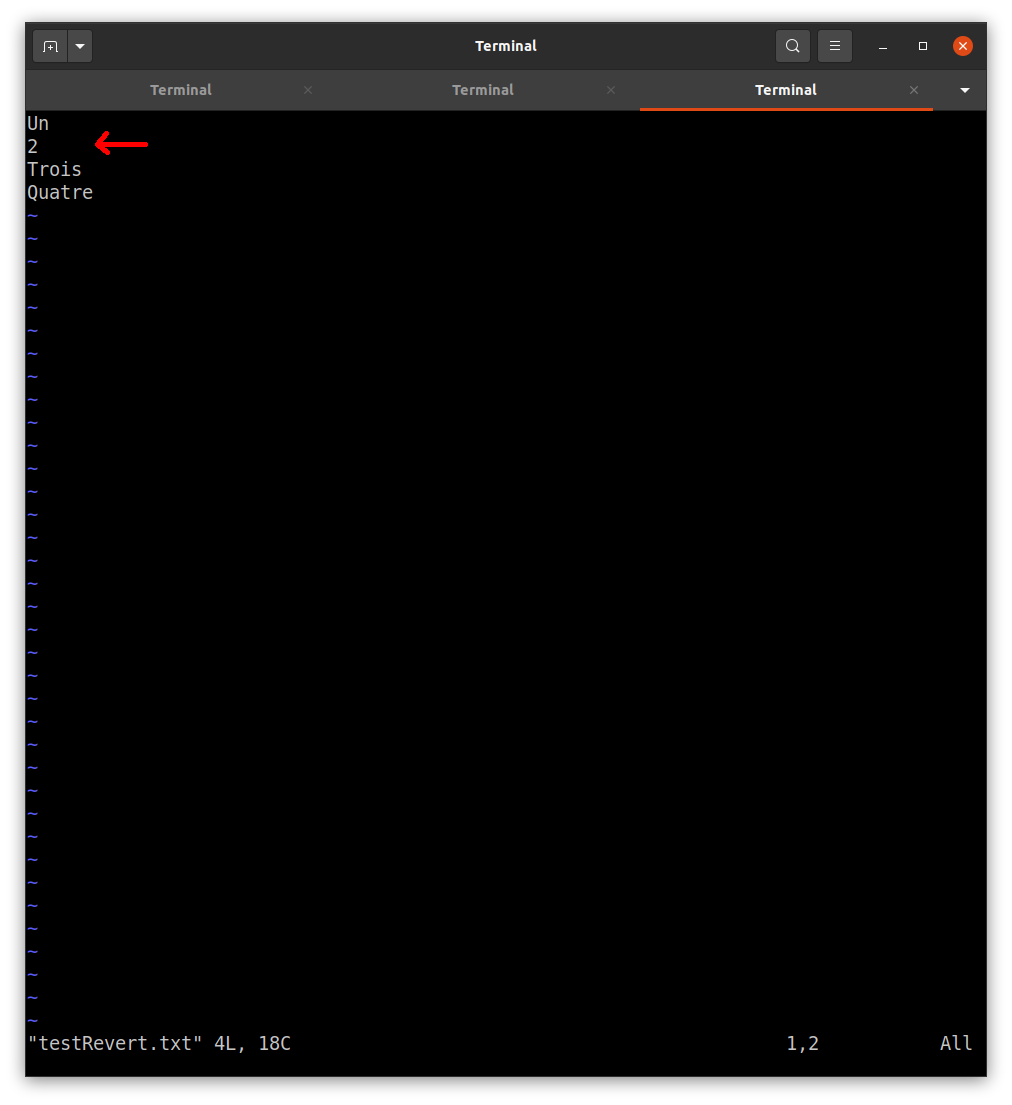
\includegraphics[scale=0.15]{gitRevert/gitRevert5.png}
\end{center}
\end{frame}

\begin{frame}{Commande: git revert <id>}
On remplace maintenant ce '2' par le mot 'DEUX' et on commit:
\begin{center}
	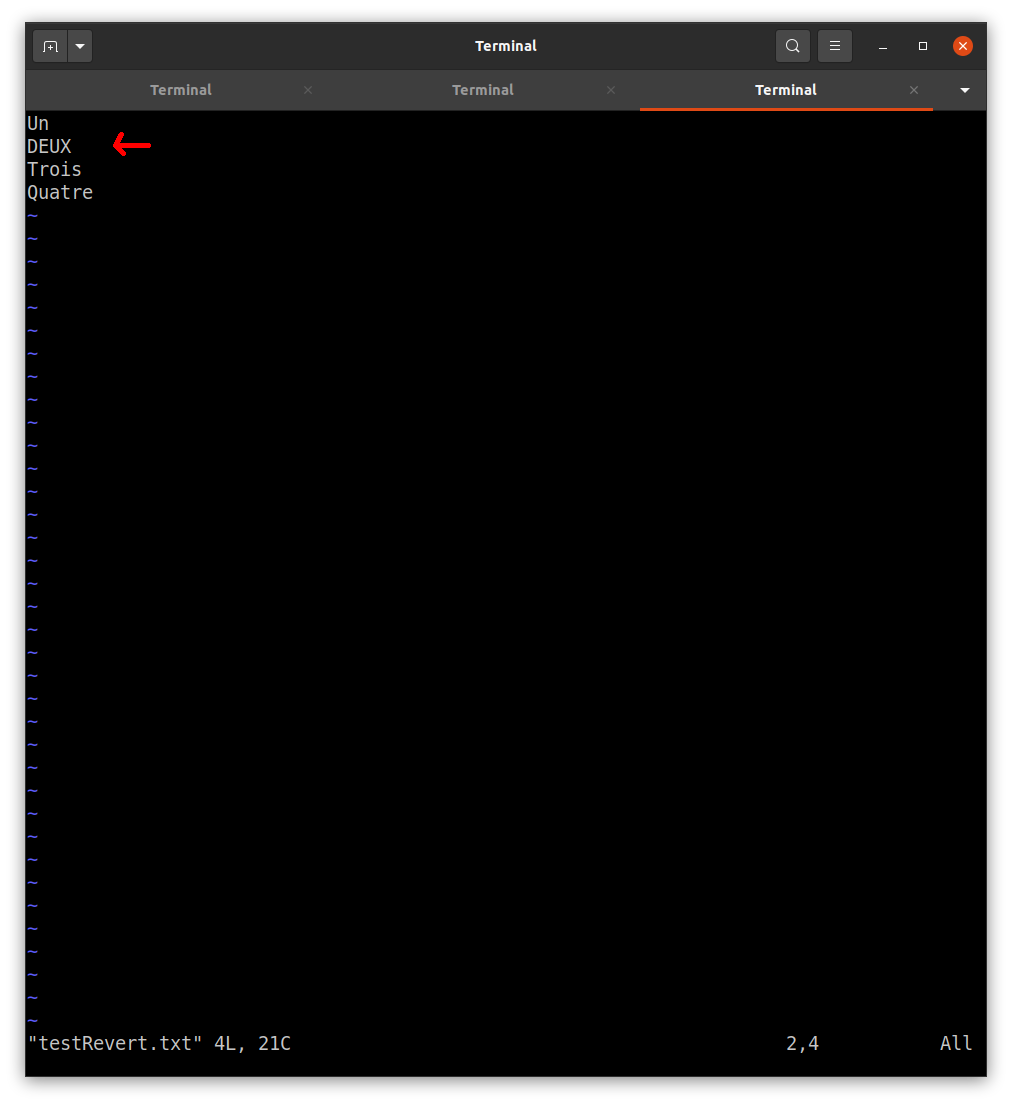
\includegraphics[scale=0.15]{gitRevert/gitRevert5b.png}
\end{center}
\end{frame}

\begin{frame}{Commande: git revert <id>}
On cherche maintenant à annuler le changement où 'Deux' a été remplacé par '2' (alors qu'on a fait un commit où '2' a été remplacé par 'DEUX'!):
\begin{center}
	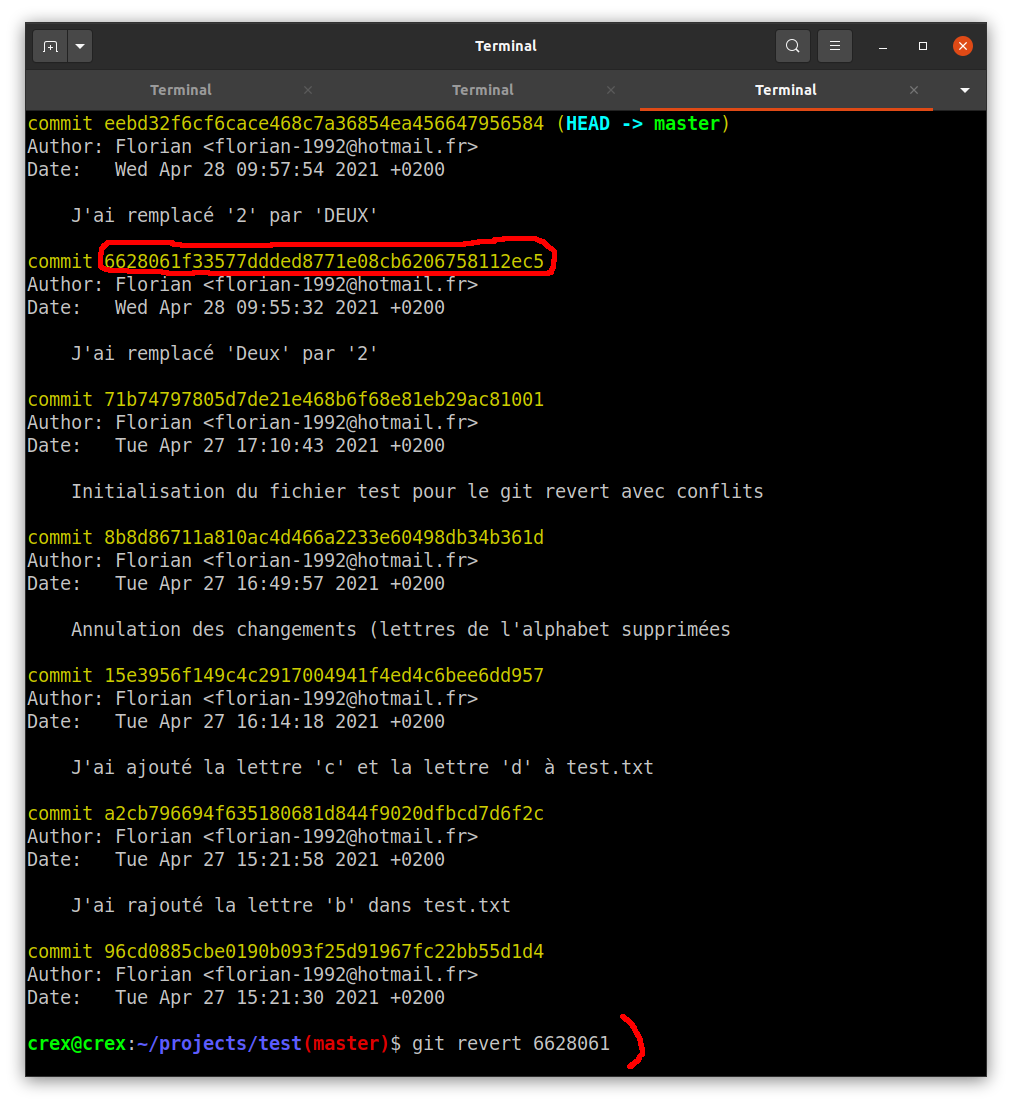
\includegraphics[scale=0.15]{gitRevert/gitRevert6.png}
\end{center}
\end{frame}

\begin{frame}{Commande: git revert <id>}
Le résultat est un conflit que nous devons résoudre à la main (exactement comme lors des conflits de collaboration):
\begin{center}
	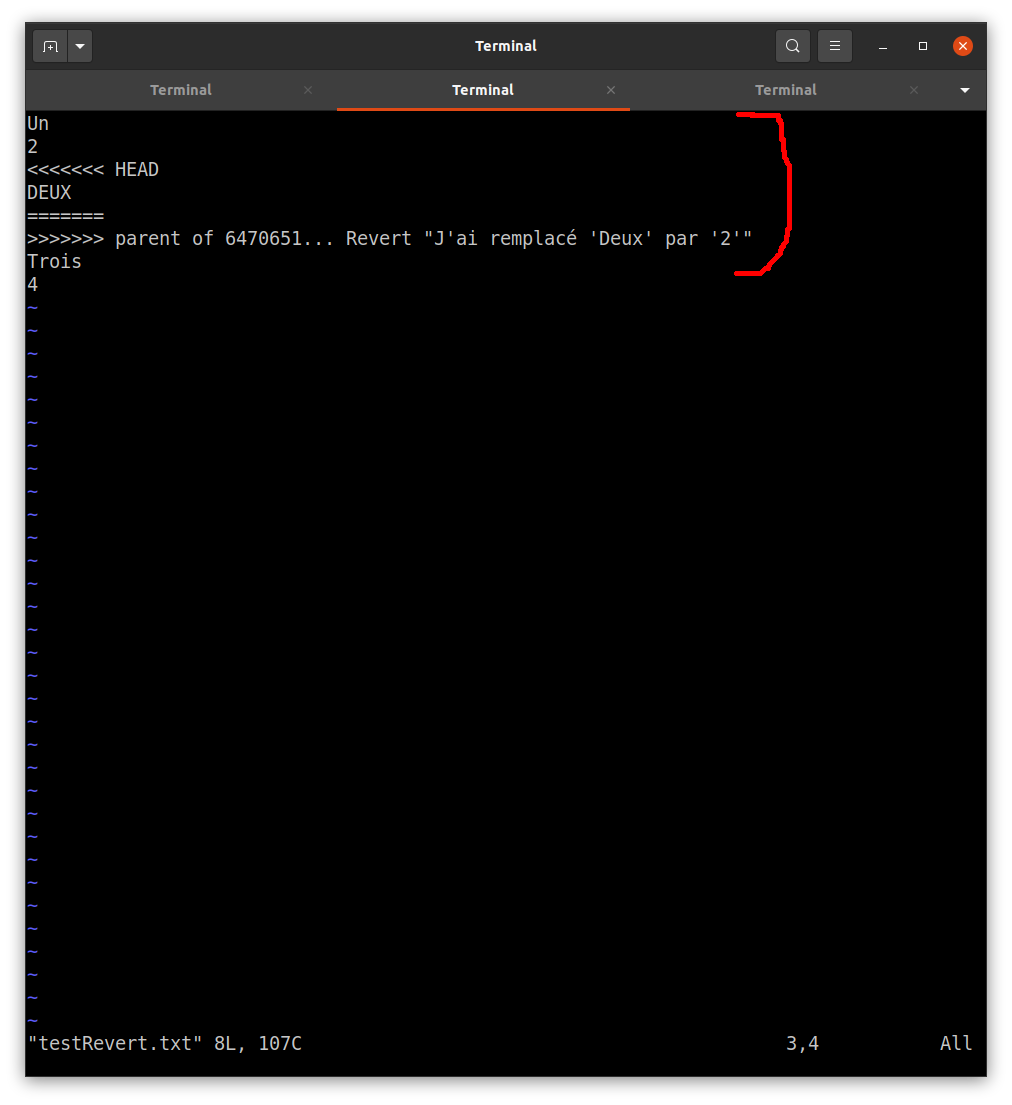
\includegraphics[scale=0.15]{gitRevert/gitRevert7.png}
\end{center}
\end{frame}

\begin{frame}{Commande: git revert <id>}
En effet, Git ne trouve pas le '2' qu'il devrait annuler. Il trouve au lieu de ça un 'DEUX' que vous avez enregistré. Or Git ne peut pas choisir entre conserver vos récentes modifications d'une part et faire l'annulation d'autre part:
\begin{center}
	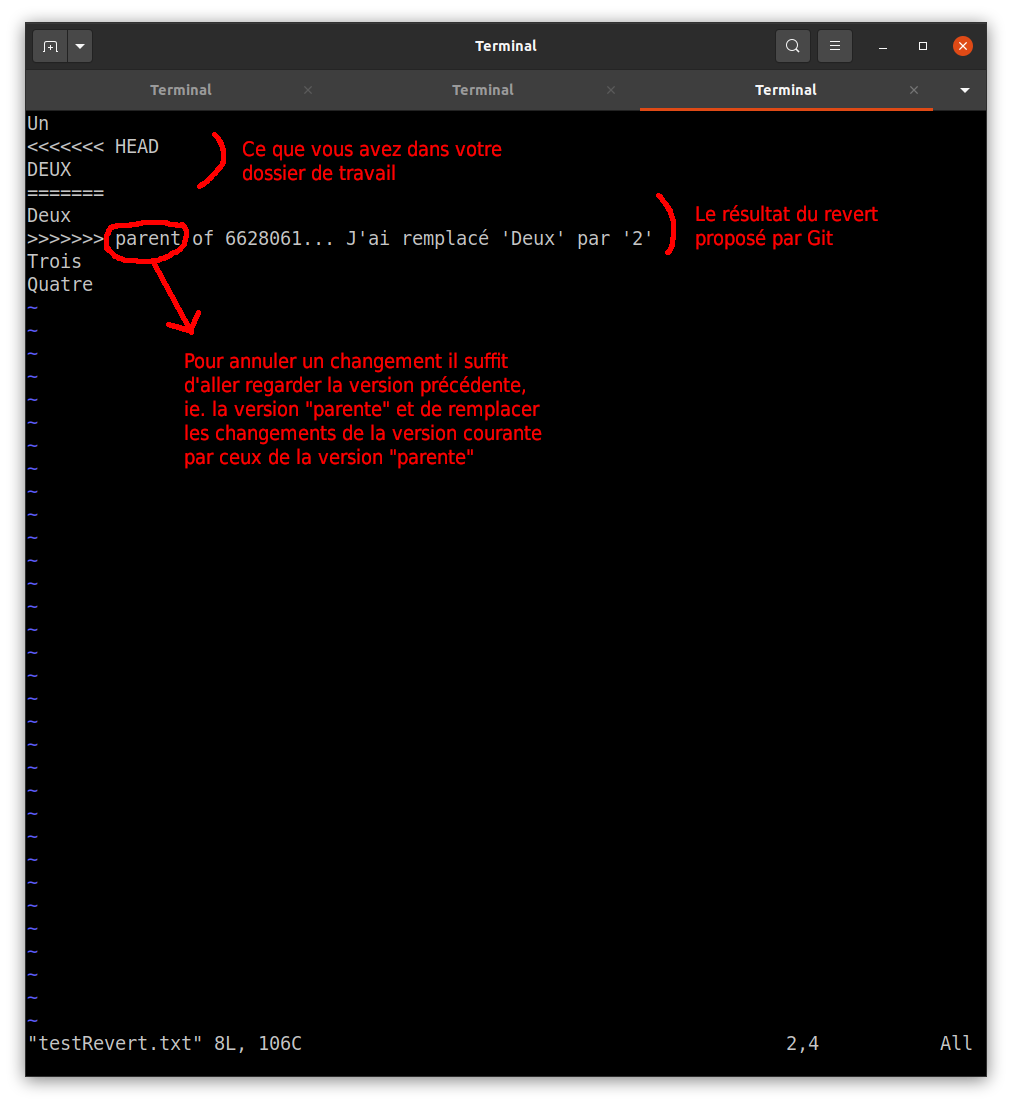
\includegraphics[scale=0.15]{gitRevert/gitRevert8.png}
\end{center}
\end{frame}

\begin{frame}{Commande: git revert <id>}
En résumé:
\begin{itemize}
	\item Tant que vous faites un \textit{git revert HEAD}, ie. tant que vous annulez votre toute dernière modification, vous n'aurez pas de conflits. En effet, pour faire un \textit{git revert <id>}, votre répertoire de travail doit être propre (sur HEAD). Les lignes que git doit annuler avec \textit{git revert HEAD} sont celles qu'ils trouvent inchangées dans votre répertoire.
	\item Si vous faites un \textit{git revert <id>} il se peut que vous ayiez des conflits à résoudre car vous aurez peut-être apporté des changements à des lignes que Git cherche à annuler et il vous demandera alors de choisir.
\end{itemize}
\end{frame}

\end{document}